% Definition of circles
\def\firstradius{(0,0) circle (1.5cm)}
\def\firstnode{(0, 0) circle (0.1cm) }

\def\secondradius{(0:2cm) circle (1.5cm)}
\def\secondnode{(0:2cm) circle (0.1cm) }

\def\midlenode {(0:1cm) circle (0.1cm) }

\colorlet{circle edge}{black!50}
\colorlet{circle area}{gray!20}

\tikzset{filled/.style={fill=circle area, draw=circle edge, thick},
    outline/.style={draw=circle edge, thick}}

\setlength{\parskip}{5mm}
% Set A and B
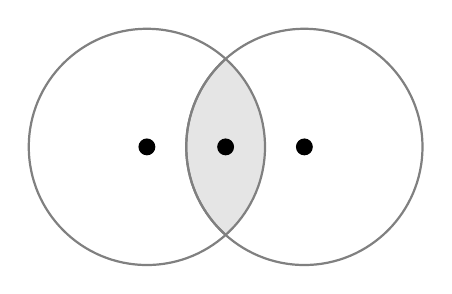
\begin{tikzpicture}
    \begin{scope}
        \clip \firstradius;
        \fill[filled] \secondradius;
        \clip \firstnode;
    \end{scope}
    
    \fill[black] \firstnode;
    \fill[black] \secondnode;
    \fill[black] \midlenode;
    
    \draw[outline] \firstradius node {};
    \draw[outline] \secondradius node {};
    
    \draw \firstnode node {};
    \draw \secondnode node {};
    \draw \midlenode node {};
%    \node[anchor=south] at (current bounding box.north) {};
\end{tikzpicture}
